\newpage
\thispagestyle{empty}
% OBS: Coloque sempre o que você quer deixar de fundo na página como primeiro comando

% Imagem de fundo - crie um arquivo separado em tamanho A4 (210x297mm) no formato pdf
\begin{tikzpicture}[remember picture,overlay]
    % Inclui a imagem em segundo plano
    \node[anchor=center,inner sep=0pt] at (current page.center) {
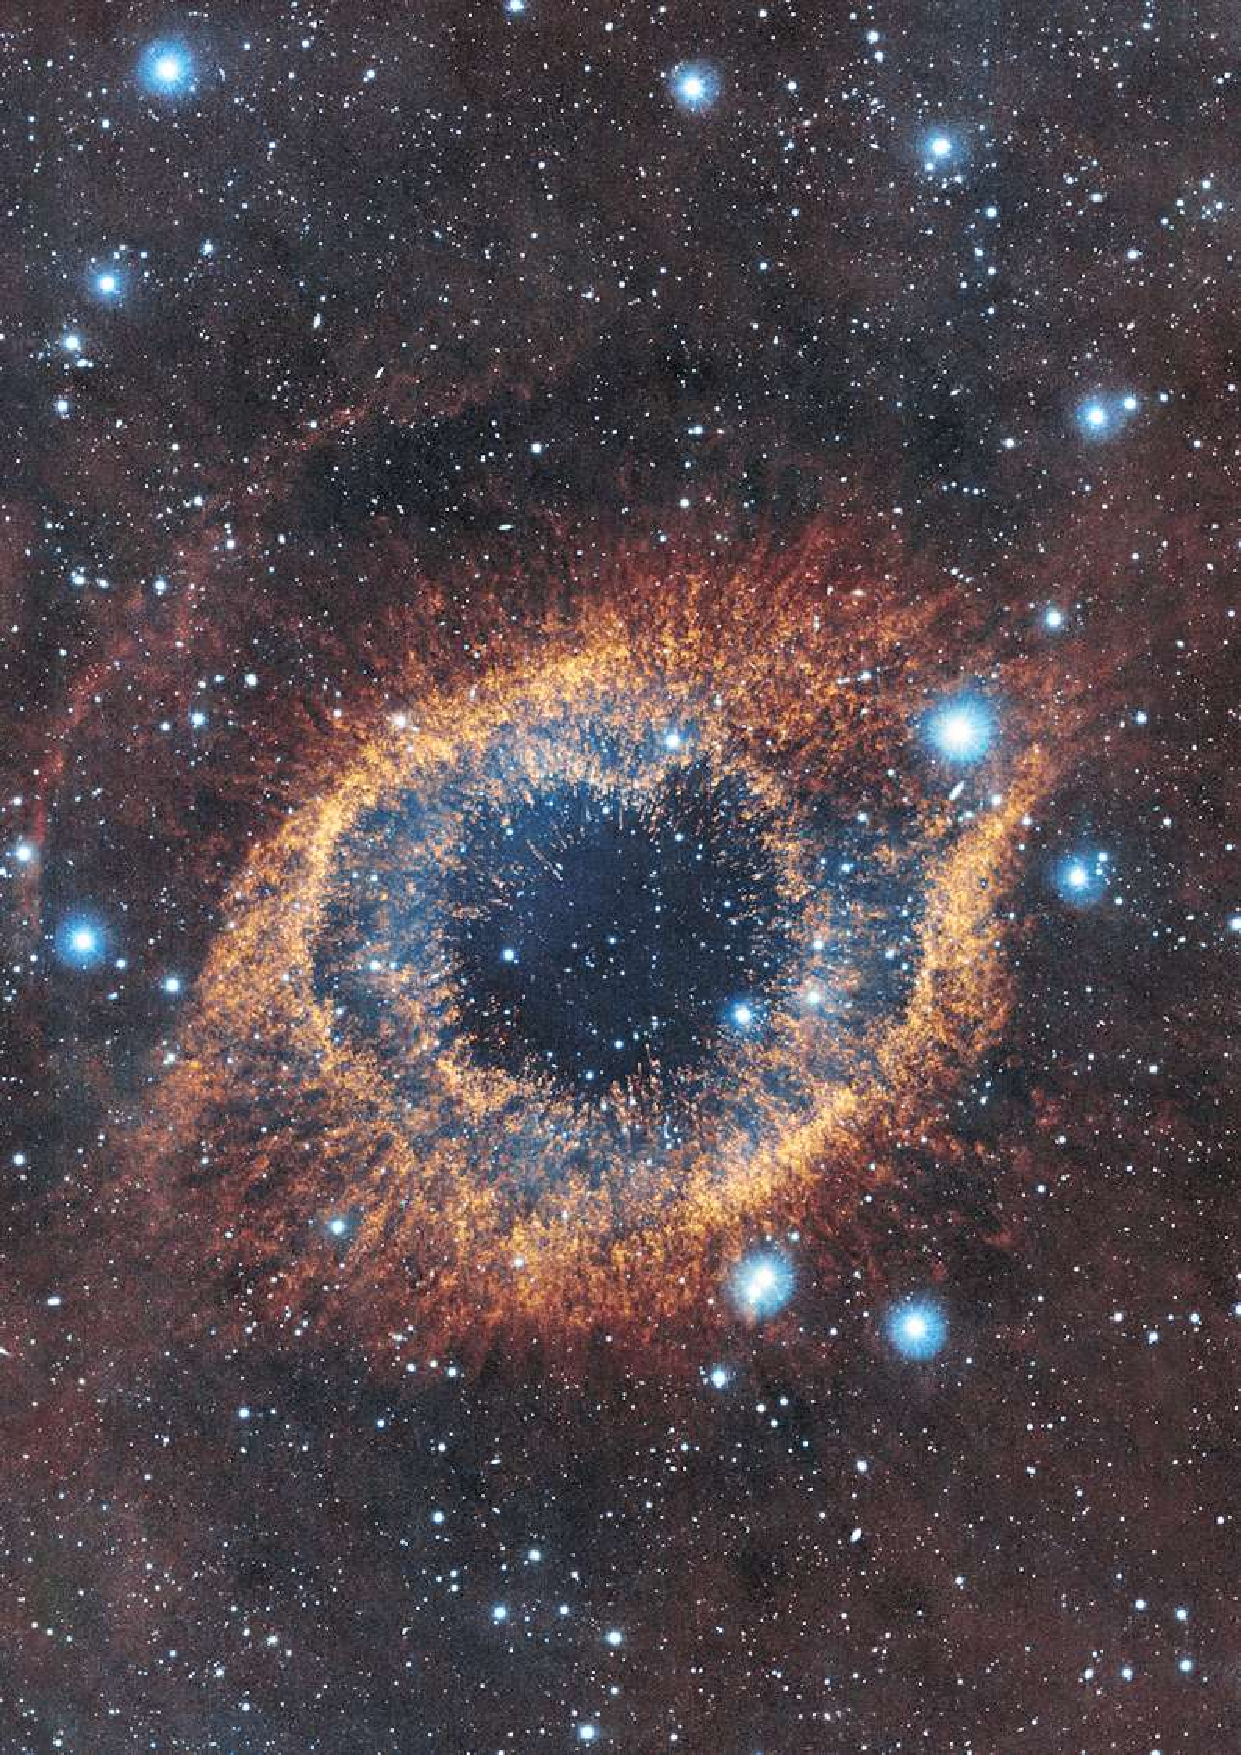
\includegraphics[width=\paperwidth,height=\paperheight,keepaspectratio]{Folha_Rosto/Figs_Folha_Rosto/HelixNebula.pdf}
    };
\end{tikzpicture}

% Marcador de página branco
\begin{tikzpicture}[remember picture, overlay, x=1.1pt, y=1.1pt, yscale=-1, xscale=1]
    % Desenho do triângulo com altura aumentada
    \begin{scope}[yshift=-3cm, xshift=-7cm]
        \draw[fill=white, draw=white] 
            (181.51,363.13) -- (181.51,-192.01) -- (390.86,-192.01) -- 
            (390.86,363.13) -- (285.98,431.63) -- (181.56,363.13) -- 
            (181.51,363.13) -- cycle;
    \end{scope}
\end{tikzpicture}

%LOGO 
% Altere a cor da logo de acordo com a cor usada para a Edição se for conveniente
\begin{tikzpicture}[remember picture, overlay]
  % Adiciona a imagem com um deslocamento usando shift
  \node at (current page.north west) [anchor=north west, xshift=3cm, yshift=-0.9cm] {
    
\includegraphics[width=7.2cm]{Folha_Rosto/Figs_Folha_Rosto/Logo_Na_Cor_Da_Edicao.png}
  };
\end{tikzpicture}

%Número da Edição, coleção (se houver) e data (mês ano)
\begin{tikzpicture}[remember picture, overlay]
  % Desenhar a primeira linha
  \draw[line width=1mm, color=base, shift={(2, -2.3)}] (-1.3,-1) -- (5.4,-1);

  % Adicionar o círculo no meio da linha com um número dentro e preenchido com a cor base
  \node[circle, draw=base, fill=base, minimum size=1cm, inner sep=0pt, text=white, shift={(2, -2.3)}] at (2,-1) {\sffamily\bfseries\myfontsizeEditionFolhaRosto \NumeroEdicao};

  % Adicionar a palavra "Coleção" entre as duas linhas
  \node[shift={(2, -2.8)}, anchor=center] at (0,-1) {\sffamily\bfseries \myfontsizeColecaoData COLEÇÃO \ColecaoEdicao};

  % Adicionar outra palavra ao lado de "Coleção"
  \node[shift={(2, -2.8)}, anchor=center] at (4,-1) {\sffamily\bfseries \myfontsizeColecaoData \MakeUppercase{\DataEdicao}};

  % Desenhar a segunda linha
  \draw[line width=1mm, color=base, shift={(2, -3.3)}] (-1.3,-1) -- (5.4,-1);

   % Desenhar uma linha pontilhada
   \foreach \i in {0.8, 0.95, 1.10, 1.25, 1.40, 1.55, 1.70, 1.85, 2, 2.15, 2.30, 2.45, 2.60, 2.75, 2.90, 3.05, 3.20} {
  \fill[base, shift={(0, -4)}] (\i+2, -1) circle (1pt);
};
  % Tema Principal
  \node[shift={(0, -5.8)}, anchor=center] at (4, -1) {
    \parbox{7cm}{\centering \sffamily\bfseries \myfontsizeColecaoTema HISTÓRIA DO\\[1.5ex]UNIVERSO:\\[1.5ex]ERA PRIMORDIAL}
  }; % Aumente o parâmetro em \parbox para caber mais texto, se for necessário
  
  % Desenhar uma linha pontilhada
   \foreach \i in {0.8, 0.95, 1.10, 1.25, 1.40, 1.55, 1.70, 1.85, 2, 2.15, 2.30, 2.45, 2.60, 2.75, 2.90, 3.05, 3.20} {
  \fill[base, shift={(0, -7.7)}] (\i+2, -1) circle (1pt);
};
  % Logo UEM
   \node[shift={(0, -9)}, anchor=center] at (4, -1) {
\includegraphics[width=0.15\textwidth]{Folha_Rosto/Figs_Folha_Rosto/UEM_Logo_Modelo_Colorido.png}
    };
\end{tikzpicture}


% Tipo do jornal
\begin{tikzpicture}[remember picture, overlay]
  % Tema Principal
  \node[shift={(4.1, -15.8)}, anchor=center] at (5.7, -1) {
    \parbox{20cm}{\sffamily\bfseries\myfontsizeDivulgacaoCientifica\textls[150]{DIVULGAÇÃO\\[0.4ex]CIENTÍFICA\\[1ex]E CULTURAL\\[1ex] PARA A\\[1ex]COMUNIDADE}}
  };
\end{tikzpicture}

